\section{Coloriages d'arêtes}
\subsection{Coloriages d'arêtes}
%il manque encore qq définitions

%dessin d'un graphe avec professeur et classes
\paragraph{Problème des horaires}
Chaque professeur doit enseigner à un certain nombre de classes pendant un certain nombre d'heures. On veut créer
un horaire sur le plus petit nombre de période possible
\\On relie chaque professeur aux classes auxquelles il donne cours en veillant a colorier les arêtes en fonction des tranches horaires. Deux arêtes de la même couleur ne peuvent pas partir du même nœud.

\index{coloriage}
\index{coloriage!coloriage d'arêtes}
\index{coloriage!coloriage d'arêtes propre}
\begin{mydef}
  Un \emph{coloriage} des arêtes d’un graphe en $k$ couleurs est l’assignation à chaque arête d’une couleur $1, 2, \ldots,$ ou $k$.
  Ce coloriage est dit \emph{propre} si deux arêtes adjacentes sont toujours de couleurs différentes.
\end{mydef}

\index{chromatique!indice chromatique}
\begin{mydef}
  L’\emph{indice chromatique} d’un graphe $G$, noté $\chi '$ ($G$) est le nombre minimal de couleurs nécessaire pour obtenir un coloriage propre des arêtes de $G$.
\end{mydef}


\begin{mytheo}[König]
  Pour tout graphe biparti: $\chi '= \degmax$
  \begin{proof}
    On va utiliser le corrolaire~\ref{corr:hall} du théorème~\ref{theo:hall} de Hall
    pour les graphes bipartis réguliers (qui ont toujours un couplage parfait).
    \begin{enumerate}
      \item Soit un graphe biparti $k$-régulier. Par le théorème de Hall, il existe un couplage parfait. On le colorie en couleur $c_{1}$. On considère ensuite les arêtes restantes non encore coloriées: elles forment un graphe $k-1$ régulier. On recommence pour la couleur $c_{2}$ avec un autre couplage. On continue jusqu'à épuisement, on obtient alors $\chi '=k$
      \item Pour un graphe biparti quelconque de degré maximum $k$.
        \begin{itemize}
          \item Ajouter des nœuds d'un côté si nécessaire pour avoir le même nombre de nœuds de chaque côté.
          \item Si tous les nœuds ne sont pas de degré $k$, alors il y a au moins 1 nœuds de degré $<k$ de chaque côté.
            On ajoute alors une arête entre eux. On recommence jusqu'à $k$-régularité.
        \end{itemize}
        Par le point 1. , il existe un coloriage propre à $k$ couleurs. On supprime ensuite les arêtes et nœuds ajoutés: on obtient un coloriage propre pour le graphe de départ.
        $$\Rightarrow \degmax \le \chi ' \le k = \degmax$$
        $$\Rightarrow \chi ' = k$$
    \end{enumerate}
  \end{proof}
\end{mytheo}

\begin{mytheo} [Vizing]
Pour tout graphe simple: $\chi ' = \degmax$ ou  $\chi ' = \degmax + 1$
  \begin{proof} On sait que $\chi' \ge \degmax$, il faut donc prouver que $\chi ' \le \degmax + 1$.
  \\On le prouve par induction sur le nombre d'arêtes du graphe.
  \\ \textbf{Pas inductif:} Vrai pour $m$ arêtes. Soit un graphe à  $m+1$ arêtes, de degré max $k$. Je retire une de ces arêtes: il existe un coloriage propre à $\le k+1$ couleurs.
  \begin{itemize}
  \item Si $\le k$ couleurs: je choisis (k+1) couleurs pour la $(m+1)^{ième}$ arête.
  \item Si $k+1$ couleurs $c_{1},...,c_{k+1}$: je rétablis la $(m+1)^{ième}$ arête: il faut trouver une couleur pour cette arête.
  \end{itemize}

  \end{proof}
\end{mytheo}
\textbf{Observation:} En chaque nœud il y a au moins une couleur libre (c'est à dire pas utilisée par les arêtes incidentes)
\\
\newline Voici 3 exemples avec $k=3$ et 4 couleurs \emph{noir, bleu, rouge et vert}
\begin{myexem} \label{exemple1}
  Même couleur libre \emph{rouge} pour $x$ et $y$ $\Rightarrow$ on peut utiliser le \emph{rouge} pour $xy$
  \begin{figure}[H]
    \begin{center}
      \subfigure[]{
        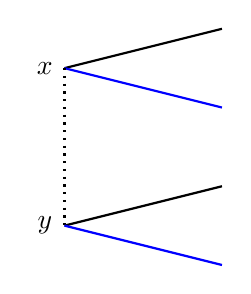
\begin{tikzpicture}[scale = 1]
          \draw[thick,black] (0,1) -- (2,1.5);
          \draw[thick,blue] (0,1) -- (2,0.5);
          \draw[thick,dotted,black] (0,1) -- (0,-1);
          \draw[thick,black] (0,-1) -- (2,-0.5);
          \draw[thick,blue] (0,-1) -- (2,-1.5);

          \node at (-0.25,1) {$x$};
          \node at (-0.25,-1){$y$};
        \end{tikzpicture}
      }
      \subfigure[]{
        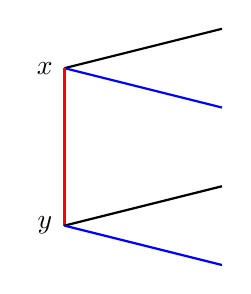
\begin{tikzpicture}[scale = 1]
          \draw[thick,black] (0,1) -- (2,1.5);
          \draw[thick,blue] (0,1) -- (2,0.5);
          \draw[very thick,red] (0,1) -- (0,-1);
          \draw[thick,black] (0,-1) -- (2,-0.5);
          \draw[thick,blue] (0,-1) -- (2,-1.5);

          \node at (-0.25,1) {$x$};
          \node at (-0.25,-1){$y$};
        \end{tikzpicture}
      }
    \end{center}
  \end{figure}
\end{myexem}

\begin{myexem}
  Pas de couleur libre entre $x$ et $y$. Mais le \emph{noir} est libre pour $y$\\
  $\Rightarrow$ on utilise le \emph{noir} pour $xy$, on efface l'arête \emph{noir} $xy'$\\
  $\Rightarrow$ On se retrouve dans le cas \ref{exemple1}, on utilise ensuite la couleur \emph{vert} pour $xy'$\\
  \begin{figure}[H]
    \begin{center}
      \subfigure[]{
        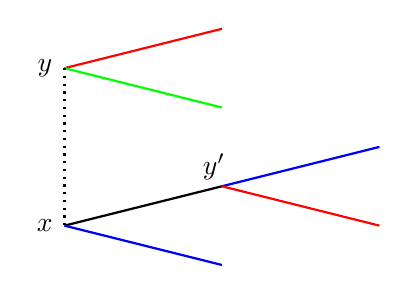
\begin{tikzpicture}[scale = 1]
          \draw[thick,red] (0,1) -- (2,1.5);
          \draw[thick,green] (0,1) -- (2,0.5);
          \draw[thick,dotted,black] (0,1) -- (0,-1);
          \draw[thick,black] (0,-1) -- (2,-0.5);
          \draw[thick,blue] (0,-1) -- (2,-1.5);
          \draw[thick,blue] (2,-0.5) -- (4,0);
          \draw[thick,red] (2,-0.5) -- (4,-1);

          \node at (-0.25,1) {$y$};
          \node at (-0.25,-1){$x$};
          \node at (1.90,-0.25){$y'$};
        \end{tikzpicture}
      }
      \subfigure[]{
        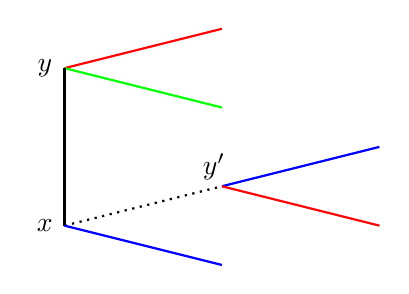
\begin{tikzpicture}[scale = 1]
          \draw[thick,red] (0,1) -- (2,1.5);
          \draw[thick,green] (0,1) -- (2,0.5);
          \draw[very thick,black] (0,1) -- (0,-1);
          \draw[thick,dotted,black] (0,-1) -- (2,-0.5);
          \draw[thick,blue] (0,-1) -- (2,-1.5);
          \draw[thick,blue] (2,-0.5) -- (4,0);
          \draw[thick,red] (2,-0.5) -- (4,-1);

          \node at (-0.25,1) {$y$};
          \node at (-0.25,-1){$x$};
          \node at (1.90,-0.25){$y'$};
        \end{tikzpicture}
      }
    \end{center}
  \end{figure}
\end{myexem}

\begin{myexem}
  Quelques fois cette astuce ne suffit pas:\\
  \begin{figure}[H]
    \begin{center}
	    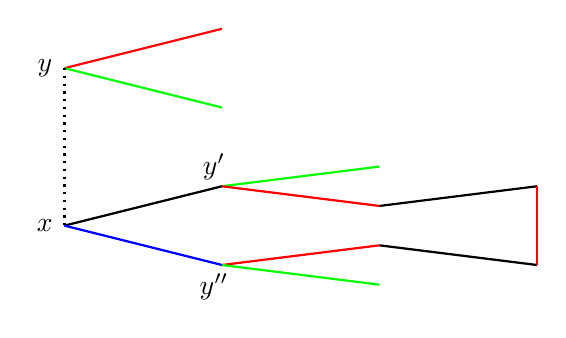
\begin{tikzpicture}[scale = 1]
        \draw[thick,red] (0,1) -- (2,1.5);
        \draw[thick,green] (0,1) -- (2,0.5);
        \draw[thick,dotted,black] (0,1) -- (0,-1);
        \draw[thick,black] (0,-1) -- (2,-0.5);
        \draw[thick,blue] (0,-1) -- (2,-1.5);
        \draw[thick,green] (2,-0.5) -- (4,-0.25);
        \draw[thick,red] (2,-0.5) -- (4,-0.75);
        \draw[thick,red] (2,-1.5) -- (4,-1.25);
        \draw[thick,green] (2,-1.5) -- (4,-1.75);
        \draw[thick,black] (4,-0.75) -- (6,-0.5);
        \draw[thick,black] (4,-1.25) -- (6,-1.5);
        \draw[thick,red] (6,-0.5) -- (6,-1.5);

        \node at (-0.25,1) {$y$};
        \node at (-0.25,-1){$x$};
        \node at (1.90,-0.25){$y'$};
        \node at (1.90,-1.78){$y''$};
      \end{tikzpicture}
    \end{center}
  \end{figure}
  Échangeons le \emph{noir} et \emph{rouge} le long du chemin des arêtes de couleurs \emph{noir} et \emph{vert} issus de $xy'$ (le coloriage reste propre) :\\
  \begin{figure}[H]
    \begin{center}
      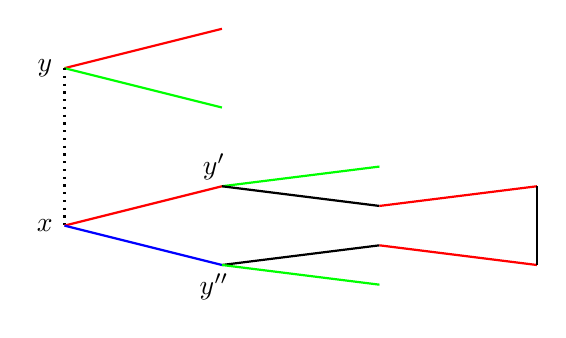
\begin{tikzpicture}[scale = 1]
        \draw[thick,red] (0,1) -- (2,1.5);
        \draw[thick,green] (0,1) -- (2,0.5);
        \draw[thick,dotted,black] (0,1) -- (0,-1);
        \draw[thick,red] (0,-1) -- (2,-0.5);
        \draw[thick,blue] (0,-1) -- (2,-1.5);
        \draw[thick,green] (2,-0.5) -- (4,-0.25);
        \draw[thick,black] (2,-0.5) -- (4,-0.75);
        \draw[thick,black] (2,-1.5) -- (4,-1.25);
        \draw[thick,green] (2,-1.5) -- (4,-1.75);
        \draw[thick,red] (4,-0.75) -- (6,-0.5);
        \draw[thick,red] (4,-1.25) -- (6,-1.5);
        \draw[thick,black] (6,-0.5) -- (6,-1.5);

        \node at (-0.25,1) {$y$};
        \node at (-0.25,-1){$x$};
        \node at (1.90,-0.25){$y'$};
        \node at (1.90,-1.78){$y''$};
      \end{tikzpicture}
    \end{center}
  \end{figure}
  $c_{1}$ libre $\Rightarrow$ même cas que: \ref{exemple1}
\end{myexem}

% FIXME L'argument ne suffit pas, il faut considérer le cas y'' = y !!
